\section{Methodology}

This section will describe the methodology to fulfill the research target. As mentioned in the \ref{aor}, the primary goal of this research is to introduce the bayesian learning method into active learning framework to handling the learning problem with variant size of data set and enable the model flexible enough to adapt the model complexity. 
\begin{figure}[htbp]
\centering
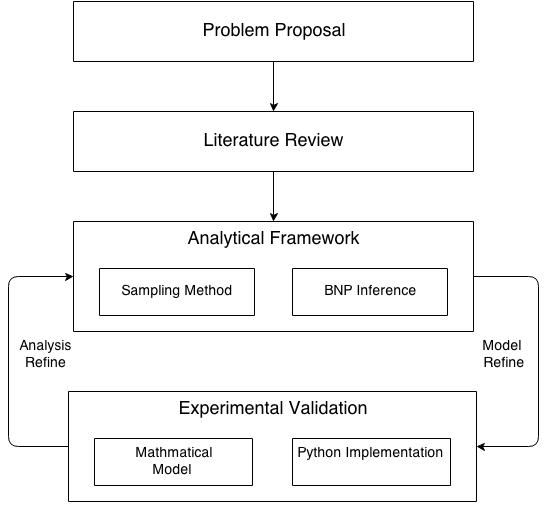
\includegraphics[width=\linewidth]{proposal}
\caption{Research Flowchart}
\label{fig:proposal}
\end{figure}

Fig\ref{fig:proposal} is the main flowchart.  briefing the detailed process, and in each main stage the major work should be:
\begin{enumerate}
 \item \textbf{Literature Review}
 
 This part should not be restricted just to the two main mentioned topics, instead during this procedure, a comprehensive review on the machine learning literature should be carried out. Besides the classical learning theories, extensive reading on analysis of their characteristics and application should also be focused on. The goal is to gain a general understanding of the theory framework, relation to other learning theory,  their history, development and current research. 
 
 \item \textbf{Develop a new sampling method in active learning}
 
 Currently, the general querying mehtods in active learning is to select either informative or representative unlabeled instances\cite{huang2010active}. It remains a challenge to select instances that are distinct on both features\cite{huang2010active}. Informativeness is the measurement of a instance on the prediction ability on the labeled data while the representativeness is the prediction ability on the unlabeled data. The current popular approaches such as query-by-committee\cite{Settles2010}, uncertainty sampling\cite{Settles2010} and so on are all under the framework of querying informative instances. The performance is greatly improved when compared to the algorithms without the active learning procedure. But all these approaches is unable to exploit the potential abundance in the unlabeled data set. Thus the aim of the research is to try to improve the efficiency by diving into the unlabeled data set while maintaining the performance on labeled dataset. This requries the sampling procedure should take into consideration both the informativeness and representativeness of an instance. Thus the new sampling method should be in the form of measuring the desired sample's representative ability in unlabeled data set and its informativeness on the change of model. We will dive into the theoretical analysis on the current different sampling scheme and try to combine them under the same framework. The effectiness of the proposed framework will be tested through experiment and the performance will be used for analysis refine.
 
 \item \textbf{Research on Bayesian Non-parametric Learning scheme}
 
 As the second main research topic, it is also very important to develop the overall learning scheme. BNP model, although very flexible and covering multiple learning tasks. The main focus on this area is how to overcome the low convergency rate in traditional BNP learning. Derived from traditional nonparametric model, Bayesian Non-parametric method is also constrained by the common shortcoming of nonparametric family, which is the high cost on resources\cite{ghosh1982nonparametric,vapnik1998statistical}. Every sample should be kept for the model updating, which will be a disaster as dimension of data set grows. In this research, we aim to bring active learning procedure into the BNP model. During the model updating, instead of storing all training samples, only those is most representative and informative will be kept. The key problem is how to make most of the selected samples in BNP learning process as all the parameters will be updated by using them.  
 \item \textbf{Implementation and Experiment}
 
 This steps include implementing the proposed framework and test the algorithm on different data set regarding the specific problem this framework will be used to evaluate its performance. The validation should contain two stage, the first one being comparison with classical and state-of-art algorithm in active learning and bayesian nonparametric model leanring respectively, the second one being test the performance of the whole framework. Currently, the most popular data set used for active learning contains:
 \begin{itemize}
 \item{\textbf{Text}}:Three data sets, 20 Newsgroups, SRAA, and Reuters-21578,have been preprocessed for an active learning setting by some researchers. The data in these data sets are categorized to a hierarchical structure. Data from different subcategories under the same parent category are considered to be from different but related domains. The task is to predict the labels of the parent category.
 \item{\textbf{E-mail}}:This data set is provided by the 2006 ECML/ PKDD discovery challenge. It is to classify the E-mail to a topic group.
 \item{\textbf{Wifi}}:This data set is provided by the ICDM-2007 Contest.
 The data were collected inside a building for localization in two
different time periods. And the purpose it to find the most probable period of the building. It is a binary classification problem.
 \end{itemize}
 
 Most of the programming will be in Python, as it is free, with many open-sourced mathimatical toolbox, and is easy to use. And the programming will be run on regular PC. 
 
 
 The result will be compared to the state-of-art methods,in the area of the problem to be solved, such as classification, regression or density estimation, on the basis of both the efficiency and accuracy. The accuracy is to test how our proposed method performs regarding to the specific target of the problem. And the efficiency is to check whether this framework will decrease the rely on calculation resource, both time and space. The performance will be the feedback for analytical refinement.
\end{enumerate}